\chapter{Example chapter}
This chapter i just to state an example create reference about some useful \LaTeX code.

\section{Code}
Check out this cool JavaScript code in \ref{code:handy_javascript}.

\begin{lstlisting}[caption=This is some handy JavaScript code, label=code:handy_javascript]
function getmbidFromURL(){
    var x = 0;
    var param = location.search;
    return param.substring(6);
}
\end{lstlisting}

\section{Images}
Here is a fancy screenshot shown in \ref{fig:example1}.

\begin{figure}[ht]
 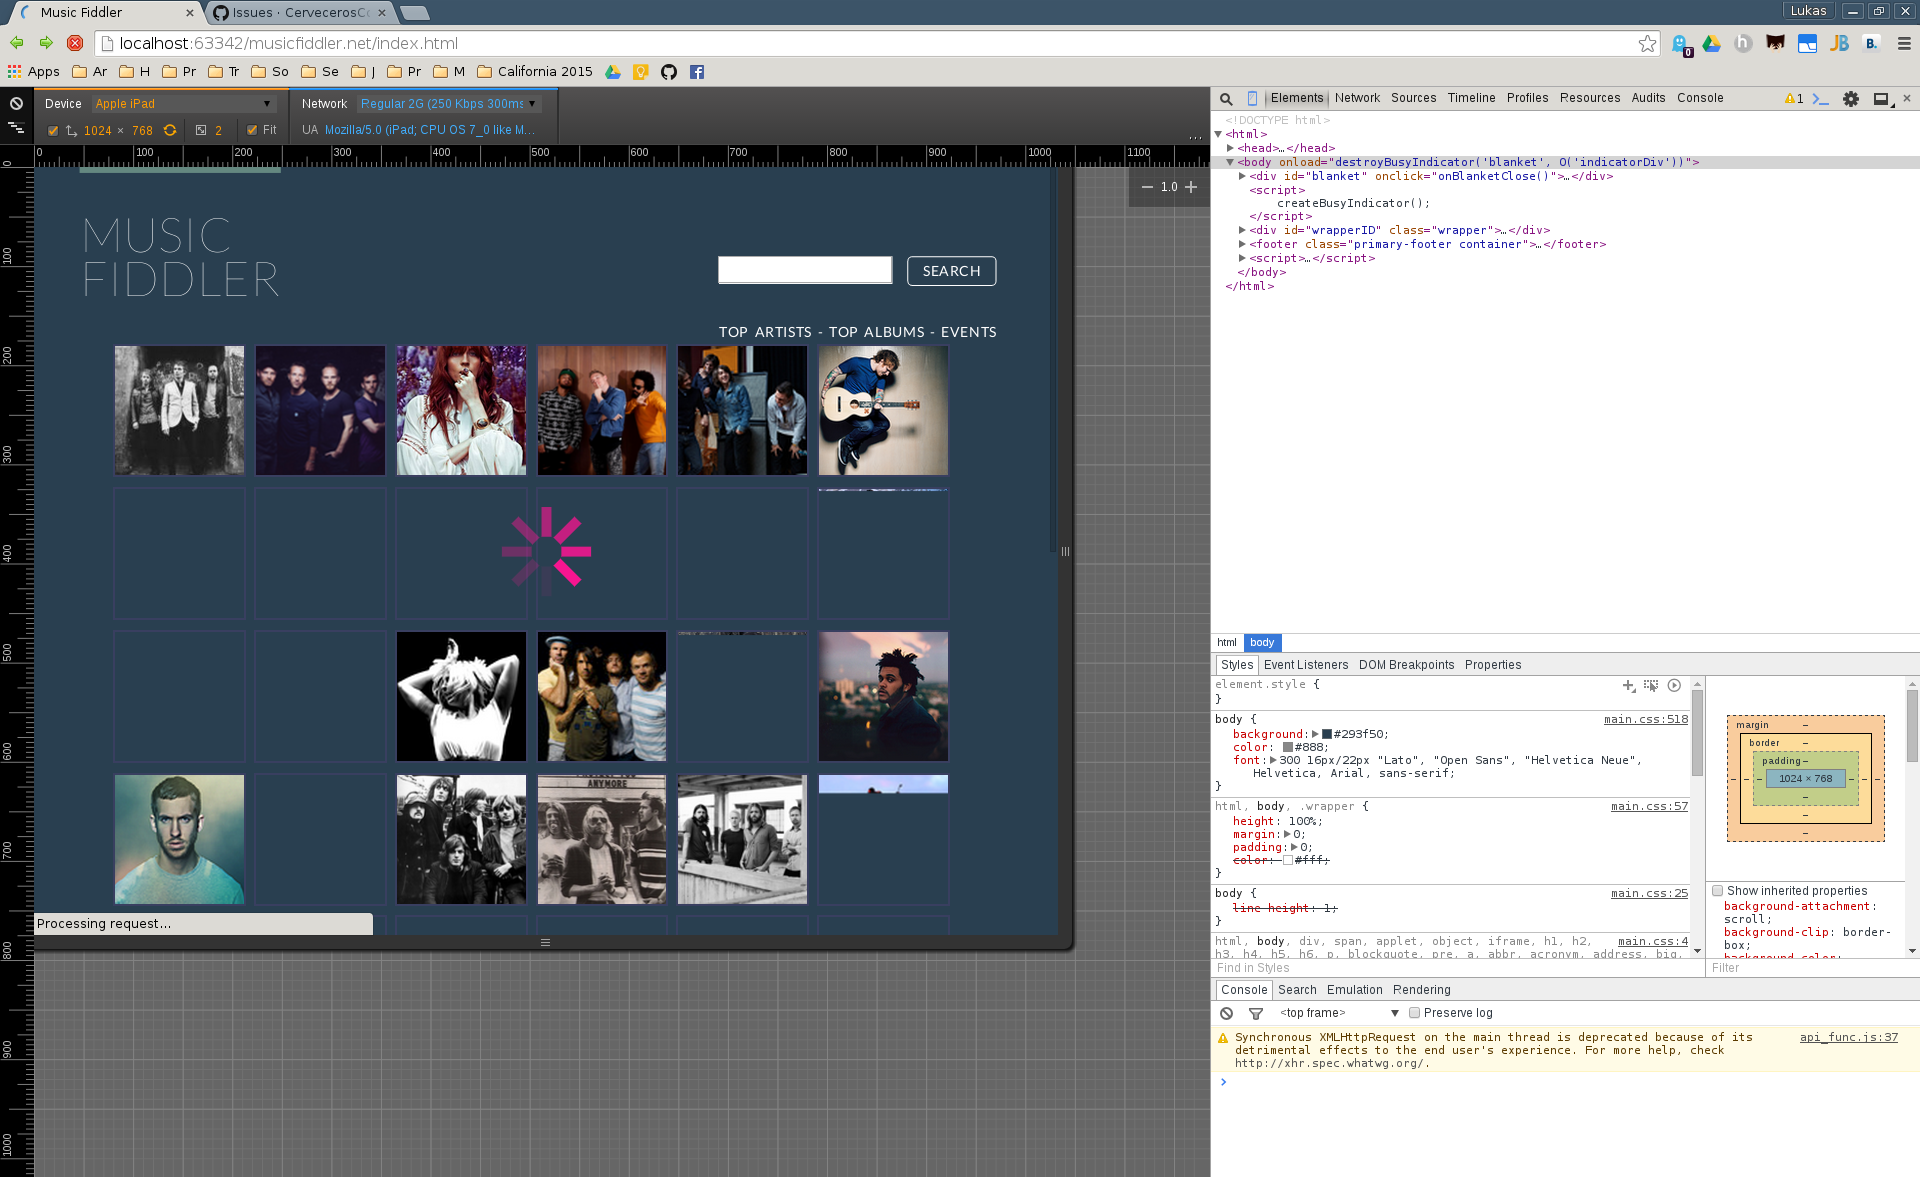
\includegraphics[width=\textwidth,height=\textheight,keepaspectratio]{./img/example/pic1.png}
 \caption[Short caption for table of contents here]{musicfiddler.net in development (this is a place for the long caption)}
 \label{fig:example1}
\end{figure}